\begin{frame}{Sparse optimization}
    \begin{tikzpicture}[remember picture,overlay]
        \begin{scope}[xshift=0.5\textwidth]
            \onslide<1-> {
                \node[text width=0.75\linewidth,align=center] at (0,3.4) {\textbf{Sparse optimization} \\ \textcolor{TolLightOrange}{Minimize} a function with a \textcolor{TolLightOrange}{sparse} solution};
            }
            %
            %
            %
            \onslide<2-> {
                \begin{scope}[yshift=40]
                \path[
                    mindmap,
                    concept color=mDarkTeal, 
                    level 1 concept/.append style={
                    minimum size    = 1.1cm,
                    text width      = 1.1cm,
                    level distance  = 3cm,
                    sibling angle   = 60,
                    font            = \scriptsize\bfseries,
                    },
                    level 2 concept/.append style={
                    minimum size    = 1.1cm,
                    text width      = 1.1cm,
                    level distance  = 2cm,
                    sibling angle   = 45,
                    font            = \scriptsize,
                    }
                ]
                node[concept,text=white,minimum size=1.6cm,text width=2.25cm] {\normalsize\textbf{Applications}}
                [clockwise from=0]
                child[concept color=TolLightRed!40] {
                    node[concept] {signal process.}
                    [clockwise from=45]
                    child { node[concept] {signal denoising} }
                    child { node[concept] {sparse decoding} }
                    child { node[concept] {phase retrieval} }
                    child { node[concept] {DOA design} }
                }  
                child[concept color=TolLightBrown!40] {
                    node[concept] {operation research}
                    [clockwise from=337.5]
                    child { node[concept] {portfolio optim.} }
                    child { node[concept] {network design} }
                    child { node[concept] {facility location} }
                }
                child[concept color=TolLightGreen!40] {
                    node[concept] {algebra}
                    [clockwise from=-67.5]
                    child { node[concept] {sparse factor.} }
                    child { node[concept] {low-rank factor.} }
                    child { node[concept] {feasible system} }
                }
                child[concept color=TolDarkBlue!40] {
                    node[concept] {statistics \& ML} 
                    [clockwise from=-90]
                    child { node[concept] {sparse PCA} }
                    child { node[concept] {sparse SVM} }
                    child { node[concept] {dictionary learning} }
                    child { node[concept] {feature selection} }
                };
                \end{scope}
                %
                \node[font=\small] at (0,-4) {A. Tillmann \textit{et. al} (2024)};
            }
        \end{scope}
    \end{tikzpicture}
\end{frame}
  
\begin{frame}{Compressed sensing}
    \begin{tikzpicture}[remember picture,overlay]
        \begin{scope}[xshift=0.5\textwidth]
            \onslide<1-> {
                \node[text width=0.25\linewidth,align=center] (groundtruth) at (-4,2.5) {Sparse signal \\ $\pv \in \kR^{\pdim}$};
                %
                \draw ($(groundtruth)+(0,-1.75)$) node {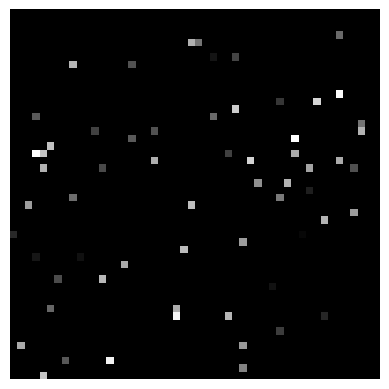
\includegraphics[width=2cm]{imgs/cs-x.png}};
                %
                \node at ($(groundtruth)+(0,-3)$) {$\pdim$ pixels};
            }
            %
            %
            %
            \onslide<2-> {
                \node[text width=0.25\linewidth,align=center] (observation) at (4,2.5) {Observation \\ $\obs = \dic\pv + \boldsymbol{\epsilon} \in \kR^{\ddim}$};
                %
                \draw[ultra thick,->] ($(groundtruth.north east)+(0,-0.25)$) .. controls (0,3.25) .. ($(observation.north west)+(0,-0.25)$) node[midway,fill=TolLightWhite,draw,ultra thick,text width=0.35\linewidth,align=center,yshift=-5] {Linear compression};
                %
                \draw ($(observation)+(0,-1.75)$) node {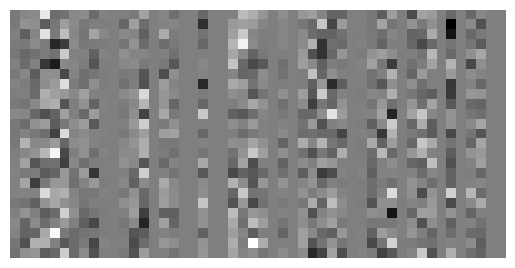
\includegraphics[width=2.5cm]{imgs/cs-y.png}};
                %
                \node at ($(observation)+(0,-2.75)$) {$\ddim$ pixels, $\ddim \ll \pdim$};
            }
            %
            %
            %
            \onslide<3-> {
                \draw[ultra thick,<-] ($(groundtruth.south east)+(0,0.25)$) .. controls (0,1.75) .. ($(observation.south west)+(0,0.25)$) node[midway,fill=TolLightWhite,draw,ultra thick,text width=0.35\linewidth,align=center,yshift=5] {Recover $\pv$ from $\dic$ and $\obs$};
            }
            %
            %
            %
            \onslide<4-> {
                \node [text width=0.45\textwidth] at (0,-1) (problem) {
                    \begin{blockcolor}{mDarkTeal}{Goal}
                    \centering
                    Find $\pv$ such that $\obs \simeq \dic\pv$
                    \end{blockcolor}
                };
            }
            %
            %
            %
            \onslide<5-> {
                \node [text width=0.45\textwidth] at ($(problem)+(0,-2.25)$) (problem-sparse) {
                    \begin{blockcolor}{mDarkTeal}{Goal}
                        \centering
                        Find $\pv$ \textcolor{TolLightOrange}{sparse} such that $\obs \simeq \dic\pv$
                    \end{blockcolor}
                };
                %
                \draw[ultra thick,->] ($(problem)+(0,-0.75)$) -- ($(problem-sparse)+(0,0.5)$) node[midway,fill=TolLightWhite,draw,ultra thick] {no unique solution};
            }
        \end{scope}
    \end{tikzpicture}
\end{frame}
  
\begin{frame}{Feature selection}
    \begin{tikzpicture}[remember picture,overlay]
        \begin{scope}[xshift=0.5\textwidth]
            \onslide<1-> {
                \node (table) at (0,1.5) {
                    \begin{tabular}{c|cccc|c}
                        \toprule
                        & \textbf{Feature 1} & \textbf{Feature 2} & $\quad$...$\quad$ & \textbf{Feature n} & $\ \ $\textbf{Target}$\ \ $ \\
                        \midrule
                        \textbf{Sample 1} & \textcolor{mDarkTeal!20}{$a_{1,1}$} & \textcolor{mDarkTeal!20}{$a_{1,2}$} & \textcolor{mDarkTeal!20}{...} & \textcolor{mDarkTeal!20}{$a_{1,\pdim}$} & \textcolor{mDarkTeal!20}{$\obsi{1}$} \\
                        \textbf{Sample 2} & \textcolor{mDarkTeal!20}{$a_{2,1}$} & \textcolor{mDarkTeal!20}{$a_{2,2}$} & \textcolor{mDarkTeal!20}{...} & \textcolor{mDarkTeal!20}{$a_{2,\pdim}$} & \textcolor{mDarkTeal!20}{$\obsi{2}$} \\
                        \textbf{Sample 3} & \textcolor{mDarkTeal!20}{$a_{3,1}$} & \textcolor{mDarkTeal!20}{$a_{3,2}$} & \textcolor{mDarkTeal!20}{...} & \textcolor{mDarkTeal!20}{$a_{3,\pdim}$} & \textcolor{mDarkTeal!20}{$\obsi{3}$} \\
                        \textcolor{mDarkTeal!20}{...} & \textcolor{mDarkTeal!20}{...} & \textcolor{mDarkTeal!20}{...} & \textcolor{mDarkTeal!20}{...} & \textcolor{mDarkTeal!20}{...} & \textcolor{mDarkTeal!20}{...} \\
                        \textbf{Sample m} & \textcolor{mDarkTeal!20}{$a_{\ddim,1}$} & \textcolor{mDarkTeal!20}{$a_{\ddim,2}$} & \textcolor{mDarkTeal!20}{...} & \textcolor{mDarkTeal!20}{$a_{\ddim,\pdim}$} & \textcolor{mDarkTeal!20}{$\obsi{\ddim}$} \\
                        \bottomrule
                    \end{tabular}
                };
                %
                \node[draw,ultra thick,fill=TolLightWhite,font=\small] (features) at ($(table.center)+(0,-0.5)$) {$\dic \in \kR^{\ddim\times\pdim}$};
                \node[draw,ultra thick,fill=TolLightWhite,font=\small] (outcome) at ($(table.center)+(4.2,-0.5)$) {$\obs \in \kR^{\ddim}$};
            }
            %
            %
            %
            \onslide<2-> {
                \node[text width=0.275\linewidth,align=center] (feature) at ($(table.south)+(-3.5,-0.6)$) {Features $\dic \in \kR^{\ddim\times\pdim}$};
                \node[text width=0.275\linewidth,align=center] (outcome) at ($(table.south)+(3.5,-0.6)$) {Target $\obs = \phi(\dic\pv)$};
                %
                \draw[ultra thick,<->] (feature) -- (outcome) node[midway,below,TolLightOrange] {weights $\pv \in \kR^{\pdim}$};
            }
            %
            %
            %
            \onslide<3-> {
                \node[font=\small,text width=0.3\linewidth,align=center] (loss) at ($(table.south)+(-1.75,-2)$) {\textbf{Model accuracy} \\ Loss $\mathcal{L}_{\phi}(\dic\pv,\obs)$};
                %
                \node[font=\small,text width=0.3\linewidth,align=center] (reg) at ($(table.south)+(1.75,-2)$) {\textbf{Model explicability} \\ Use few features};
            }
            %
            %
            %
            \onslide<4-> {
                \draw[ultra thick,->] (loss) -- ($(loss)+(0,-0.75)$);
                \draw[ultra thick,->] (reg) -- ($(reg)+(0,-0.75)$);
                %
                \node[align=center,text width=0.6\textwidth] (serm) at ($(table.south)+(0,-3.25)$) {
                    \begin{blockcolor}{mDarkTeal}{Goal}
                    \centering
                    Find $\pv$ \textcolor{TolLightOrange}{sparse} such that $\mathcal{L}_{\phi}(\dic\pv,\obs)$ is small 
                    \end{blockcolor}
                };
            }
        \end{scope}
    \end{tikzpicture}
\end{frame}
  
\begin{frame}{Network design}
    \begin{tikzpicture}[remember picture,overlay]
        \begin{scope}[xshift=0.5\textwidth]
        
            \coordinate (A) at (-3.5,1);
            \coordinate (B) at ($(A)+(2,0)$);
            \coordinate (C) at ($(A)+(1,2)$);
            \coordinate (D) at ($(A)+(1,-2)$);
            \coordinate (E) at ($(A)+(3,1)$);
            \coordinate (F) at ($(A)+(3,-1)$);
            \coordinate (G) at ($(A)+(-1,1.5)$);
            \coordinate (H) at ($(A)+(-1,-1.5)$);
            \coordinate (I) at ($(A)+(4,0)$);
            \coordinate (J) at ($(A)+(-2,0)$);

            \draw[ultra thick,dashed] (A) -- (B);
            \draw[ultra thick,dashed] (A) -- (C);
            \draw[ultra thick,dashed] (A) -- (D);
            \draw[ultra thick,dashed] (A) -- (G);
            \draw[ultra thick,dashed] (A) -- (H);
            \draw[ultra thick,dashed] (B) -- (C);
            \draw[ultra thick,dashed] (B) -- (D);
            \draw[ultra thick,dashed] (B) -- (E);
            \draw[ultra thick,dashed] (B) -- (F);
            \draw[ultra thick,dashed] (B) -- (I);
            \draw[ultra thick,dashed] (C) -- (E);
            \draw[ultra thick,dashed] (C) -- (G);
            \draw[ultra thick,dashed] (D) -- (F);
            \draw[ultra thick,dashed] (D) -- (H);
            \draw[ultra thick,dashed] (E) -- (I);
            \draw[ultra thick,dashed] (F) -- (I);
            \draw[ultra thick,dashed] (G) -- (H);
            \draw[ultra thick,dashed] (G) -- (J);
            \draw[ultra thick,dashed] (H) -- (J);

            \node[ultra thick, circle, draw, minimum size=6mm, fill=TolLightWhite] at (A) {};
            \node[ultra thick, circle, draw, minimum size=6mm, fill=TolLightWhite] at (B) {};
            \node[ultra thick, circle, draw, minimum size=6mm, TolLightRed, fill=TolLightWhite] at (C) {\small\textcolor{TolLightRed}{\textbf{3}}};
            \node[ultra thick, circle, draw, minimum size=6mm, TolLightRed, fill=TolLightWhite] at (D) {\small\textcolor{TolLightRed}{\textbf{3}}};
            \node[ultra thick, circle, draw, minimum size=6mm, fill=TolLightWhite] at (E) {};
            \node[ultra thick, circle, draw, minimum size=6mm, fill=TolLightWhite] at (F) {};
            \node[ultra thick, circle, draw, minimum size=6mm, fill=TolLightWhite] at (G) {};
            \node[ultra thick, circle, draw, minimum size=6mm, fill=TolLightWhite] at (H) {};
            \node[ultra thick, circle, draw, minimum size=6mm, TolLightRed, fill=TolLightWhite] at (I) {\small\textcolor{TolLightRed}{\textbf{3}}};
            \node[ultra thick, circle, draw, minimum size=6mm, TolLightBlue, fill=TolLightWhite] at (J) {\small\textcolor{TolLightBlue}{\textbf{9}}};

            \node[text width=0.6\linewidth,align=center] at (-2.5,-2) {Which edges to build to transport products from \textcolor{TolLightBlue}{source} to \textcolor{TolLightRed}{sink} nodes ?};


            \node[ultra thick, circle, draw, minimum size=6mm, fill=TolLightWhite] (N1) at (2.5,1) {};
            \node[ultra thick, circle, draw, minimum size=6mm, fill=TolLightWhite] (N2) at (4.5,1) {};
            \draw[ultra thick,dashed] (N1) -- (N2);
            \node[text width=0.5\linewidth,align=center,anchor=north] at ($(N1)!0.5!(N2)+(0,-0.5)$) {construction cost $c$ per edge \\ transportation cost $Q(\pv)$ \\ capacity $\0 \leq \pv \leq \mathbf{x}_{\text{ub}}$ \\ flow conservation $\mathbf{D}\pv \leq \mathbf{d}$};

            % \node[text width=0.35\linewidth,align=center] at (9,1) {
            %   \begin{blockcolor}{mDarkTeal}{Network design}
            %       \centering
            %       $\textstyle
            %       \left\{
            %           \begin{array}{rl}
            %               \min & Q(\pv) + \reg\norm{\pv}{0} \\ 
            %               \text{s.t.} & \mathbf{D}\pv \leq \mathbf{d}, \ \pv \leq \mathbf{c} \\ & \pv \in \kR+^{\card(E)}
            %           \end{array}
            %       \right.$
            %   \end{blockcolor}
            % };
            % \node[text width=0.5\linewidth,align=left] at (10.5,-2) {\begin{itemize}[nosep]\item[$Q$ :] transportation cost \item[$\reg$ :] unit construction cost \item[$\mathbf{D}\pv \leq \mathbf{d}$ :] flow conservation \item[$\0 \leq \pv \leq \mathbf{c}$ :] capacity constraint\end{itemize}};
        \end{scope}
    \end{tikzpicture}
\end{frame}
  
\begin{frame}{Minimized, constrained, or regularized problem ?}
    \begin{tikzpicture}[remember picture,overlay]
        \begin{scope}[xshift=0.5\textwidth]
            \onslide<1-> {
                \node[text width=0.75\linewidth,align=center] (sparse) at (0,3.4) {\textbf{Sparse optimization} \\ \textcolor{TolLightOrange}{Minimize} a function with a \textcolor{TolLightOrange}{sparse} solution};
            }
            %
            %
            %
            \onslide<2-> {
                \node[text width=0.35\textwidth,align=center] (loss) at (-3,1) {$\lfunc(\pv)$ \\ thing to minimize};
                %
                % \draw[ultra thick] ($(sparse)+(-3.2,-0.4)$) -- ($(sparse)+(-3.2,-0.5)$) -- ($(sparse)+(-0.15,-0.5)$) -- ($(sparse)+(-0.15,-0.4)$);
                %
                \draw [ultra thick,->] ($(sparse)+(-1.5,-0.5)$) -- (loss) node[midway,fill=TolLightWhite,draw,ultra thick] {quantify cost};
            }
            %
            %
            %
            \onslide<3-> {
                \node[text width=0.35\textwidth,align=center] (norm) at (3,1) {$\norm{\pv}{0}$ \\ counts non-zeros};
                %
                % \draw[ultra thick] ($(sparse)+(3.2,-0.4)$) -- ($(sparse)+(3.2,-0.5)$) -- ($(sparse)+(0.9,-0.5)$) -- ($(sparse)+(0.9,-0.4)$);
                %
                \draw [ultra thick,->] ($(sparse)+(1.5,-0.5)$) -- (norm) node[midway,fill=TolLightWhite,draw,ultra thick] {quantify sparsity};
            }
            %
            %
            %
            \onslide<4-> {
                \node[text width=0.45\textwidth] at (-3,-1) {
                \begin{blockcolor}{mDarkTeal}{\textbf{Constrained version}}
                    \centering
                    $\begin{array}{ll} \min_{\pv \in \kR^{\pdim}} & \ \lfunc(\pv) \\ \text{subject to} & \ \norm{\pv}{0} \leq s\end{array}$
                \end{blockcolor}
                };
            }
            %
            %
            %
            \onslide<5-> {
                \node[text width=0.45\textwidth] at (3,-1) {
                \begin{blockcolor}{mDarkTeal}{\textbf{Minimized version}}
                    \centering
                    $\begin{array}{ll} \min_{\pv \in \kR^{\pdim}} & \ \norm{\pv}{0} \\ \text{subject to} & \ \lfunc(\pv) \leq \epsilon\end{array}$
                \end{blockcolor}
                };
            }
            %
            %
            %
            \onslide<6-> {
                \node[text width=0.45\textwidth] at (0,-3.25) {
                \begin{blockcolor}{mDarkTeal}{\textbf{Regularized version}}
                    \centering
                    $\min_{\pv \in \kR^{\pdim}} \lfunc(\pv) + \reg\norm{\pv}{0} + \textcolor{TolLightOrange}{\pfunc(\pv)}$
                \end{blockcolor}
                };
            }
        \end{scope}
    \end{tikzpicture}
\end{frame}
  
\begin{frame}{A bit of history}
    \begin{tikzpicture}[remember picture,overlay]
        \begin{scope}[xshift=0.5\textwidth]
            \onslide<1-> {
                \node[align=center,text width=0.45\textwidth] (problem) at (0,3) {
                    \begin{blockcolor}{mDarkTeal}{Problem}
                        \centering
                        $\min_{\pv \in \kR^{\pdim}} \lfunc(\pv) + \reg\norm{\pv}{0} + \pfunc(\pv)$
                    \end{blockcolor}
                };
                %
                \node at ($(problem.south)+(0,-0.1)$) {NP-hard to solve};
            }
            %
            %
            %
            \onslide<2-> {
                \node (linecenter) at ($(current page.north)+(0,-0.55\textheight)$) {};
                \draw [ultra thick,->] ($(linecenter)+(-6,0)$) -- ($(linecenter)+(6,0)$) node (arrow) [midway] {};
                %
                \node (date1) at ($(linecenter)+(-5,0)$) {};
                \draw [ultra thick,-] ($(date1)+(0,-0.02\textheight)$) -- ($(date1)+(0,0.02\textheight)$);
                \node at ($(date1)+(0,+0.06\textheight)$)  {\textbf{1995}};
                \node[text width=0.2\textwidth,align=center,font=\small] at ($(date1)+(0,-0.05\textheight)$) {Heuristics};
                \node[text width=0.3\textwidth,align=center,font=\scriptsize] at ($(date1)+(0,-0.12\textheight)$) {MP, OMP, ... \\ S. Mallat (1993)};
                %
                \node (origin1) at ($(date1)+(0,-0.4\textheight)$) {};
                \fill[draw,thick,fill=TolLightWhite] ($(origin1)+(-0.5,0)$) circle (0.1);
                \fill[draw,thick,fill=TolLightOrange] ($(origin1)+(-0.5,0.3)$) circle (0.1);
                \fill[draw,thick,fill=TolLightWhite] ($(origin1)+(-0.5,0.6)$) circle (0.1);
                \fill[draw,thick,fill=TolLightWhite] ($(origin1)+(-0.5,0.9)$) circle (0.1);
                \fill[draw,thick,fill=TolLightWhite] ($(origin1)+(-0.5,1.2)$) circle (0.1);
                \fill[draw,thick,fill=TolLightWhite] ($(origin1)+(-0.5,1.5)$) circle (0.1);
                \node at ($(origin1)+(-0.5,-0.4)$) {$\pv^1$};
                %
                \fill[draw,thick,fill=TolLightWhite] ($(origin1)+(0,0)$) circle (0.1);
                \fill[draw,thick,fill=TolLightOrange] ($(origin1)+(0,0.3)$) circle (0.1);
                \fill[draw,thick,fill=TolLightWhite] ($(origin1)+(0,0.6)$) circle (0.1);
                \fill[draw,thick,fill=TolLightOrange] ($(origin1)+(0,0.9)$) circle (0.1);
                \fill[draw,thick,fill=TolLightWhite] ($(origin1)+(0,1.2)$) circle (0.1);
                \fill[draw,thick,fill=TolLightWhite] ($(origin1)+(0,1.5)$) circle (0.1);
                \node at ($(origin1)+(0,-0.4)$) {$\pv^2$};
                %
                \fill[draw,thick,fill=TolLightWhite] ($(origin1)+(0.5,0)$) circle (0.1);
                \fill[draw,thick,fill=TolLightOrange] ($(origin1)+(0.5,0.3)$) circle (0.1);
                \fill[draw,thick,fill=TolLightWhite] ($(origin1)+(0.5,0.6)$) circle (0.1);
                \fill[draw,thick,fill=TolLightOrange] ($(origin1)+(0.5,0.9)$) circle (0.1);
                \fill[draw,thick,fill=TolLightOrange] ($(origin1)+(0.5,1.2)$) circle (0.1);
                \fill[draw,thick,fill=TolLightWhite] ($(origin1)+(0.5,1.5)$) circle (0.1);
                \node at ($(origin1)+(0.5,-0.4)$) {$\pv^3$};
            }
            %
            %
            %
            \onslide<3-> {
                \node (date2) at ($(linecenter)+(-2.5,0)$) {};
                \draw [ultra thick,-] ($(date2)+(0,-0.02\textheight)$) -- ($(date2)+(0,0.02\textheight)$);
                \node at ($(date2)+(0,+0.06\textheight)$)  {\textbf{2000}};
                \node[text width=0.25\textwidth,align=center,font=\small] at ($(date2)+(0,-0.053\textheight)$) {Recovery cond.};
                \node[text width=0.3\textwidth,align=center,font=\scriptsize] at ($(date2)+(0,-0.12\textheight)$) {RIP, NSP, ... \\ E. Candes (2004)};
                %
                \node (origin2) at ($(date2)+(0,-0.4\textheight)$) {};
                \node[text width=0.2\linewidth,align=center,font=\small] at ($(origin2)+(0,0.065\textheight)$) {OMP solves $\ell_0$-problem under RIP};
            }
            %
            %
            %
            \onslide<4-> {
                \node (date3) at ($(linecenter)+(0,0)$) {};
                \draw [ultra thick,-] ($(date3)+(0,-0.02\textheight)$) -- ($(date3)+(0,0.02\textheight)$);
                \node at ($(date3)+(0,+0.06\textheight)$)  {\textbf{2005}};
                \node[font=\small] at ($(date3)+(0,-0.053\textheight)$) {Convex approx.};
                \node[text width=0.3\textwidth,align=center,font=\scriptsize] at ($(date3)+(0,-0.12\textheight)$) {Lasso, Elastic-Net, ... \\ R. Tibshirani (2005)};
                %
                \node (origin3) at ($(date3)+(0,-0.4\textheight)$) {};
                \draw[ultra thick,->] ($(origin3)+(-1,0)$) -- ($(origin3)+(1, 0)$);
                \draw[ultra thick,->] ($(origin3)+(0,0)$) -- ($(origin3)+(0,1.5)$);
                \draw[-,very thick,TolLightOrange] ($(origin3)+(-0.05,0.8)$) -- ($(origin3)+(-1,0.8)$);
                \draw[-,very thick,TolLightOrange] ($(origin3)+(0.05,0.8)$) -- ($(origin3)+(1,0.8)$);
                \draw[very thick,dashed,TolLightOrange] (origin3) .. controls ($(origin3)+(-0.5,0.1)$) ..  ($(origin3)+(-1,0.8)$);
                \draw[very thick,dashed,TolLightOrange] (origin3) .. controls ($(origin3)+(0.5,0.1)$) ..  ($(origin3)+(1,0.8)$);
                \draw[TolLightOrange,very thick] ($(origin3)+(0,0.8)$) circle (0.075);
                \fill[TolLightOrange] (origin3) circle (0.075);
            }
            %
            %
            %
            \onslide<5-> {
                \node (date4) at ($(linecenter)+(2.5,0)$) {};
                \draw [ultra thick,-] ($(date4)+(0,-0.02\textheight)$) -- ($(date4)+(0,0.02\textheight)$);
                \node at ($(date4)+(0,+0.06\textheight)$)  {\textbf{2010}};
                \node[font=\small] at ($(date4)+(0,-0.053\textheight)$) {Concave approx.};
                \node[text width=0.3\textwidth,align=center,font=\scriptsize] at ($(date4)+(0,-0.12\textheight)$) {SCAD, MCP, ... \\ C. Zhang (2010)};
                %
                \node (origin4) at ($(date4)+(0,-0.4\textheight)$) {};
                \draw[ultra thick,->] ($(origin4)+(-1,0)$) -- ($(origin4)+(1, 0)$);
                \draw[ultra thick,->] ($(origin4)+(0,0)$) -- ($(origin4)+(0,1.5)$);
                \draw[-,very thick,TolLightOrange] ($(origin4)+(-0.05,0.8)$) -- ($(origin4)+(-1,0.8)$);
                \draw[-,very thick,TolLightOrange] ($(origin4)+(0.05,0.8)$) -- ($(origin4)+(1,0.8)$);
                \draw[very thick,TolLightOrange,dashed] (origin4) .. controls ($(origin4)+(-0.5,0.8)$) ..  ($(origin4)+(-1,0.8)$);
                \draw[very thick,TolLightOrange,dashed] (origin4) .. controls ($(origin4)+(0.5,0.8)$) ..  ($(origin4)+(1,0.8)$);
                \draw[TolLightOrange,very thick] ($(origin4)+(0,0.8)$) circle (0.075);
                \fill[TolLightOrange] (origin4) circle (0.075);
            }
            %
            %
            %
            \onslide<6-> {
                \node (date5) at ($(linecenter)+(5,0)$) {};
                \draw[ultra thick,-] ($(date5)+(0,-0.02\textheight)$) -- ($(date5)+(0,0.02\textheight)$);
                \node at ($(date5)+(0,+0.06\textheight)$)  {\textbf{2015}};
                \node[text width=0.22\textwidth,align=center,font=\small,TolLightOrange] at ($(date5)+(0,-0.05\textheight)$) {Exact methods};
                \node[text width=0.3\textwidth,align=center,font=\scriptsize] at ($(date5)+(0,-0.12\textheight)$) {MIP, BnB, ... \\ D. Bertsimas (2016)};
                %
                \node (origin5) at ($(date5)+(0,-0.4\textheight)$) {};
                \draw[ultra thick,->] ($(origin5)+(-1,0)$) -- ($(origin5)+(1, 0)$);
                \draw[ultra thick,->] ($(origin5)+(0,0)$) -- ($(origin5)+(0,1.5)$);
                \draw[-,very thick,TolLightOrange] ($(origin5)+(-0.05,0.8)$) -- ($(origin5)+(-1,0.8)$);
                \draw[-,very thick,TolLightOrange] ($(origin5)+(0.05,0.8)$) -- ($(origin5)+(1,0.8)$);
                \draw[TolLightOrange,very thick] ($(origin5)+(0,0.8)$) circle (0.075);
                \fill[TolLightOrange] (origin5) circle (0.075);
            }
        \end{scope}
    \end{tikzpicture}
\end{frame}
  
\begin{frame}{Complexity-tractability balance}
    \AddTodo{Slide, tell what's my point with this talk}
\end{frame}